% Provenance (never printed): see sources/outline_sources.md (Year 3:
% critical-taper theory; fold-and-thrust belts; exhumation and
% thermochronology). Brief: sources/book5/BRIEFS.md, ch. 10. Curves from
% figdata/bachelor-3/fault_bend.py, critical_taper.py and age_elevation.py.
% Exercise and problem values in the Book 5 scratch calculator calc/ch10.py.
\chapter{Chaînes de chevauchement et prismes orogéniques}\label{ch:b3:orogenic-wedges}

Lorsqu'on pousse un bulldozer dans du sable humide ou de la neige, un coin de matériau
s'accumule devant la lame. Il se déforme jusqu'à ce que sa surface atteigne une certaine pente~;
il glisse alors vers l'avant d'un seul tenant et croît en gardant la même forme,
en incorporant du nouveau matériau à son pied. Les parties externes des chaînes de montagnes, de
Taïwan aux contreforts des Alpes, se comportent de la même manière~: ce sont des coins de roches
arrachées à une plaque et poussées sur une base faible, et leur pente de surface
et le pendage de leur base renseignent sur la faiblesse de cette base et sur la
pression de fluide interstitiel. Ce chapitre construit la géométrie des chaînes
de chevauchement, la mécanique du prisme et les horloges qui mesurent la vitesse
à laquelle ses roches remontent jusqu'à la surface.
% ledger: dsd83:taper

\begin{recall}
Les chevauchements, la vergence et la géométrie des plis sont traités dans le volume de première année, dans son chapitre
consacré aux failles, aux plis et aux fabriques~; le critère de Coulomb, la loi de Byerlee, la
contrainte effective et le rapport de pression interstitielle $\lambda = P/\sigma_v$ figurent dans son
chapitre sur les contraintes, la déformation et la rhéologie~; la température de fermeture et
l'âge de refroidissement figurent dans son chapitre sur les méthodes de datation radiométrique. Le décollement, la
chaîne de plis et de chevauchements, la tectonique de couverture et la tectonique de socle, ainsi que la
coupe équilibrée sont traités dans le volume de deuxième année, dans son chapitre
sur l'anatomie d'une chaîne de montagnes~; l'exhumation et sa vitesse figurent dans son chapitre sur les
chemins P--T--t. La construction par kinks et l'aire excédentaire $A = Sh$ d'un pli situé
au-dessus d'un décollement sont traitées au \cref{ch:b3:structural-analysis}~; le \omterm{def:b3:lithosphere-thermal-models:peclet}{nombre de Péclet thermique}
est traité au \cref{ch:b3:lithosphere-thermal-models}.
\end{recall}

\section{La géométrie des chevauchements}\label{sec:b3:orogenic-wedges:geometry}

Un chevauchement ne recoupe pas une série stratifiée suivant un seul plan rectiligne.
Il suit une couche faible, un schiste ou une évaporite, sur de longues distances, puis
remonte abruptement à travers les couches résistantes sus-jacentes jusqu'à la couche faible suivante.
L'escalier qu'il dessine contrôle les plis du toit.

\begin{definition}[Rampe, palier, duplex, chevauchement hors séquence]\label{def:b3:orogenic-wedges:thrust-geometry}
Un \emph{palier}\index{palier} est un segment de chevauchement qui s'étend
parallèlement à la stratification, le plus souvent dans une couche faible~; une \emph{rampe}\index{rampe}
est un segment qui recoupe la stratification,
d'environ 20 à \ang{30}, et relie un palier inférieur à un palier supérieur. Un
\emph{duplex}\index{duplex} est un empilement de tranches limitées par des failles,
appelées écailles, enserrées entre un chevauchement inférieur et un chevauchement
supérieur, chaque écaille étant limitée par une rampe qui les relie. Les chevauchements
se forment en général dans l'ordre, chaque nouveau chevauchement se formant dans le mur du précédent, plus près de
l'avant-pays~; un \emph{chevauchement hors séquence}\index{chevauchement hors séquence} est
un chevauchement qui se forme ou rejoue derrière le front actif, en recoupant les chevauchements plus anciens.
\end{definition}

Lorsque le toit franchit une courbure de la faille, il doit se plisser pour rester au
contact de celle-ci~: un synclinal se forme à l'entrée de la \omterm{def:b3:orogenic-wedges:thrust-geometry}{rampe} et un anticlinal
à sa sortie.

\begin{definition}[Plis de rampe, plis de propagation de faille et plis de décollement]\label{def:b3:orogenic-wedges:thrust-folds}
Un \emph{pli de rampe}\index{pli de rampe} est un pli du toit d'un chevauchement
formé lorsqu'il glisse au-dessus d'une courbure de la faille, c'est-à-dire d'une \omterm{def:b3:orogenic-wedges:thrust-geometry}{rampe} reliant
deux \omterm{def:b3:orogenic-wedges:thrust-geometry}{paliers}. Un \emph{pli de propagation de faille}\index{pli de propagation de faille}
se développe au-dessus de la pointe d'un chevauchement qui se propage encore vers le haut~: le
raccourcissement que la faille ne porte plus est absorbé par le plissement situé devant
sa pointe, ce qui donne un flanc frontal raide ou déversé. Un \emph{pli de
décollement}\index{pli de décollement} croît au-dessus d'un \omterm{def:b3:orogenic-wedges:thrust-geometry}{palier} sans \omterm{def:b3:orogenic-wedges:thrust-geometry}{rampe}~: le
raccourcissement est absorbé par le plissement et par une couche faible, de sel ou de schiste, qui
flue vers son cœur.
\end{definition}

La figure ci-dessous construit un \omterm{def:b3:orogenic-wedges:thrust-folds}{pli de rampe}. Ici, le toit se déplace parallèlement
au segment de faille situé dessous et se plisse selon des surfaces axiales qui
bissectent chaque courbure, modèle cinématique dit d'écoulement parallèle à la faille~; le
modèle classique à épaisseur et longueur de couche constantes donne le même
anticlinal à sommet plat, mais à flanc frontal plus raide, au prix d'une construction plus longue
(ici admise). Les deux modèles sont soumis à la conservation de l'aire.

\begin{omfigure}
\begin{tikzpicture}
\begin{groupplot}[group style={group size=1 by 2, vertical sep=0.9cm},
  width=0.92\linewidth, axis equal image,
  xmin=0, xmax=12, ymin=-0.6, axis lines=none, clip=true,
  title style={font=\small, at={(0.0,1.0)}, anchor=south west}]
% (a) before slip
\nextgroupplot[title={(a) avant glissement}, ymax=1.75]
\fill[omLithSand!70] (axis cs:0,0) rectangle (axis cs:12,1.6);
\fill[gray!25] (axis cs:0,-0.6) rectangle (axis cs:12,0);
\draw[black!70] (axis cs:0,0.25) -- (axis cs:12,0.25);
\draw[black!70] (axis cs:0,0.5) -- (axis cs:12,0.5);
\draw[black!70] (axis cs:0,0.75) -- (axis cs:12,0.75);
\draw[black!70] (axis cs:0,1.0) -- (axis cs:12,1.0);
\draw[black!70] (axis cs:0,1.3) -- (axis cs:12,1.3);
\draw[black!70] (axis cs:0,1.6) -- (axis cs:12,1.6);
\draw[black!70] (axis cs:0,-0.3) -- (axis cs:12,-0.3);
\addplot[very thick, red!70!black] table[x=x, y=y] {figdata/out/bachelor-3-fault_bend-fault.dat};
\node[font=\scriptsize, fill=omLithSand!70, inner sep=1pt] at (axis cs:2,0.125) {palier inférieur};
\node[font=\scriptsize, fill=omLithSand!70, inner sep=1pt, rotate=30] at (axis cs:4.55,0.62) {rampe};
\node[font=\scriptsize, fill=omLithSand!70, inner sep=1pt] at (axis cs:9,0.875) {palier supérieur};
% (b) after a slip of 2.5 units
\nextgroupplot[title={(b) après glissement~: un pli de rampe}, ymax=2.75]
\fill[gray!25] (axis cs:0,-0.6) rectangle (axis cs:12,0) -- cycle;
\addplot[name path=fault, draw=none] table[x=x, y=y] {figdata/out/bachelor-3-fault_bend-fault.dat};
\addplot[name path=top, draw=none] table[x=x, y=y] {figdata/out/bachelor-3-fault_bend-bed6.dat};
\addplot[name path=base, draw=none] coordinates {(0,-0.6) (12,-0.6)};
\addplot[omLithSand!70] fill between[of=fault and top];
\addplot[gray!25] fill between[of=base and fault];
\addplot[black!70] table[x=x, y=y] {figdata/out/bachelor-3-fault_bend-bed1.dat};
\addplot[black!70] table[x=x, y=y] {figdata/out/bachelor-3-fault_bend-bed2.dat};
\addplot[black!70] table[x=x, y=y] {figdata/out/bachelor-3-fault_bend-bed3.dat};
\addplot[black!70] table[x=x, y=y] {figdata/out/bachelor-3-fault_bend-bed4.dat};
\addplot[black!70] table[x=x, y=y] {figdata/out/bachelor-3-fault_bend-bed5.dat};
\addplot[black!70] table[x=x, y=y] {figdata/out/bachelor-3-fault_bend-bed6.dat};
\draw[black!70] (axis cs:4.4330,0.25) -- (axis cs:12,0.25);
\draw[black!70] (axis cs:4.8660,0.5) -- (axis cs:12,0.5);
\draw[black!70] (axis cs:5.2990,0.75) -- (axis cs:12,0.75);
\draw[black!70] (axis cs:0,-0.3) -- (axis cs:12,-0.3);
\addplot[very thick, red!70!black] table[x=x, y=y] {figdata/out/bachelor-3-fault_bend-fault.dat};
\draw[densely dashed, black!60] (axis cs:0,1.6) -- (axis cs:12,1.6);
\node[font=\scriptsize, anchor=south] at (axis cs:2.2,1.65) {surface régionale};
\node[font=\scriptsize, anchor=west] at (axis cs:8.6,2.25) {aire excédentaire $A = Sr$};
\draw[black!70] (axis cs:8.6,2.25) -- (axis cs:6.6,2.0);
\node[font=\scriptsize, fill=gray!25, inner sep=1pt] at (axis cs:10.6,0.625) {mur};
\end{groupplot}
\end{tikzpicture}

\par\smallskip{\small (a) Un chevauchement à \omterm{def:b3:orogenic-wedges:thrust-geometry}{palier} inférieur, une \omterm{def:b3:orogenic-wedges:thrust-geometry}{rampe} au pendage de
\ang{30} et un \omterm{def:b3:orogenic-wedges:thrust-geometry}{palier} supérieur, avant glissement (schéma, échelles verticale et horizontale
égales). (b) Le même après un glissement de 2.5 fois la hauteur de la \omterm{def:b3:orogenic-wedges:thrust-geometry}{rampe},
calculé par écoulement parallèle à la faille~: un synclinal au pied de la \omterm{def:b3:orogenic-wedges:thrust-geometry}{rampe}, un flanc
arrière parallèle à la \omterm{def:b3:orogenic-wedges:thrust-geometry}{rampe}, une crête plane soulevée de la hauteur de la \omterm{def:b3:orogenic-wedges:thrust-geometry}{rampe} $r$, un
flanc avant, et une aire excédentaire $Sr$ au-dessus du niveau régional de chaque couche
située au-dessus du \omterm{def:b3:orogenic-wedges:thrust-geometry}{palier} supérieur.}\label{fig:b3:orogenic-wedges:thrusts}
\end{omfigure}


\begin{proposition}[Aire excédentaire d'un pli de rampe]\label{prop:b3:orogenic-wedges:fault-bend-area}
Soit un chevauchement qui fait remonter son toit sur une \omterm{def:b3:orogenic-wedges:thrust-geometry}{rampe} de hauteur $r$, depuis un \omterm{def:b3:orogenic-wedges:thrust-geometry}{palier}
inférieur jusqu'à un \omterm{def:b3:orogenic-wedges:thrust-geometry}{palier} supérieur, le glissement $S$ étant mesuré sur le \omterm{def:b3:orogenic-wedges:thrust-geometry}{palier} inférieur. Pour toute couche du
toit située au-dessus du \omterm{def:b3:orogenic-wedges:thrust-geometry}{palier} supérieur, l'aire délimitée entre la
couche plissée et son niveau d'origine vaut $A = Sr$, la même pour chacune de ces couches.
\end{proposition}

\begin{proof}
La roche n'est ni créée ni détruite, et son volume se conserve. Prenons une coupe
parallèle au glissement, bornée par deux verticales, l'une loin à l'arrière et l'autre loin en
avant de la \omterm{def:b3:orogenic-wedges:thrust-geometry}{rampe}. Par la ligne arrière, le toit compris entre le
\omterm{def:b3:orogenic-wedges:thrust-geometry}{palier} inférieur et une couche située à la hauteur $y_0$ au-dessus de lui a avancé de $S$ dans la coupe~: l'aire
$Sy_0$ est entrée. Par la ligne avant, la roche comprise entre le \omterm{def:b3:orogenic-wedges:thrust-geometry}{palier} supérieur
et la même couche, d'épaisseur $y_0 - r$, est sortie sous l'effet du glissement sur le \omterm{def:b3:orogenic-wedges:thrust-geometry}{palier} supérieur,
également $S$ si la roche conserve son aire~: l'aire $S(y_0 - r)$
a quitté la coupe. La différence, $Sr$, est restée entre les deux lignes et soulève
la couche au-dessus de son niveau d'origine.
\end{proof}

L'aire excédentaire d'un \omterm{def:b3:orogenic-wedges:thrust-folds}{pli de rampe} mesure le glissement multiplié par la hauteur de
la \omterm{def:b3:orogenic-wedges:thrust-geometry}{rampe}, et non la profondeur du décollement, comme ce serait le cas pour un
\omterm{def:b3:orogenic-wedges:thrust-folds}{pli de décollement} (voir le \cref{ch:b3:structural-analysis}). Les deux types de plis
doivent être distingués avant qu'une aire soit convertie en raccourcissement.


Un \omterm{def:b3:orogenic-wedges:thrust-geometry}{duplex} (figure ci-dessous) se développe lorsque le chevauchement, au lieu d'entraîner son toit toujours
plus loin le long de la même \omterm{def:b3:orogenic-wedges:thrust-geometry}{rampe}, l'abandonne et recoupe dans son mur une nouvelle \omterm{def:b3:orogenic-wedges:thrust-geometry}{rampe}
en avant de l'ancienne. La tranche comprise entre l'ancienne et la nouvelle \omterm{def:b3:orogenic-wedges:thrust-geometry}{rampe} devient une
écaille, remontée sur la nouvelle \omterm{def:b3:orogenic-wedges:thrust-geometry}{rampe} et empilée sous le toit~; la \omterm{def:b3:orogenic-wedges:thrust-geometry}{rampe} suivante
se forme de nouveau en avant. Chaque écaille est raccourcie de sa longueur initiale à la
longueur qu'elle occupe désormais le long du chevauchement de base, et le raccourcissement du \omterm{def:b3:orogenic-wedges:thrust-geometry}{duplex} est
la somme de ses écailles. Les \omterm{def:b3:orogenic-wedges:thrust-geometry}{chevauchements hors séquence} rompent cet ordre~: ils se forment
lorsque le prisme situé derrière le front doit s'épaissir, cas que la mécanique de la
section suivante prédit.

\begin{omfigure}
\begin{tikzpicture}
\begin{axis}[width=0.92\linewidth, axis equal image, xmin=0, xmax=12, ymin=-0.6, ymax=1.95,
  axis lines=none, clip=true]
\fill[gray!25] (axis cs:0,-0.6) rectangle (axis cs:12,0);
\fill[omLithSand!70] (axis cs:0,0) -- (axis cs:1.0,0) -- (axis cs:2.35,1.15) -- (axis cs:12,1.15) -- (axis cs:12,1.85) -- (axis cs:2.35,1.85) -- (axis cs:1.0,0.7) -- (axis cs:0,0.7) -- cycle;
\draw[black!70] (axis cs:0,0.35) -- (axis cs:1.0,0.35) -- (axis cs:2.35,1.5) -- (axis cs:12,1.5);
\draw[black!70] (axis cs:0,0.7) -- (axis cs:1.0,0.7) -- (axis cs:2.35,1.85) -- (axis cs:12,1.85);
\fill[omLithShale!60] (axis cs:8.2,0) -- (axis cs:12,0) -- (axis cs:12,1.15) -- (axis cs:9.55,1.15) -- cycle;
\draw[black!70] (axis cs:8.646,0.38) -- (axis cs:12,0.38);
\draw[black!70] (axis cs:9.104,0.77) -- (axis cs:12,0.77);
\fill[omLithLime] (axis cs:1.0,0) -- (axis cs:2.80,0) -- (axis cs:4.15,1.15) -- (axis cs:2.35,1.15) -- cycle;
\draw[black!70] (axis cs:1.45,0) -- (axis cs:2.80,1.15);
\draw[black!70] (axis cs:1.90,0) -- (axis cs:3.25,1.15);
\draw[black!70] (axis cs:2.35,0) -- (axis cs:3.70,1.15);
\fill[omLithShale] (axis cs:2.8,0) -- (axis cs:4.60,0) -- (axis cs:5.95,1.15) -- (axis cs:4.15,1.15) -- cycle;
\draw[black!70] (axis cs:3.25,0) -- (axis cs:4.60,1.15);
\draw[black!70] (axis cs:3.70,0) -- (axis cs:5.05,1.15);
\draw[black!70] (axis cs:4.15,0) -- (axis cs:5.50,1.15);
\fill[omLithLime] (axis cs:4.6,0) -- (axis cs:6.40,0) -- (axis cs:7.75,1.15) -- (axis cs:5.95,1.15) -- cycle;
\draw[black!70] (axis cs:5.05,0) -- (axis cs:6.40,1.15);
\draw[black!70] (axis cs:5.50,0) -- (axis cs:6.85,1.15);
\draw[black!70] (axis cs:5.95,0) -- (axis cs:7.30,1.15);
\fill[omLithShale] (axis cs:6.4,0) -- (axis cs:8.20,0) -- (axis cs:9.55,1.15) -- (axis cs:7.75,1.15) -- cycle;
\draw[black!70] (axis cs:6.85,0) -- (axis cs:8.20,1.15);
\draw[black!70] (axis cs:7.30,0) -- (axis cs:8.65,1.15);
\draw[black!70] (axis cs:7.75,0) -- (axis cs:9.10,1.15);
\draw[thick, red!70!black] (axis cs:1.0,0) -- (axis cs:2.35,1.15);
\draw[thick, red!70!black] (axis cs:2.8,0) -- (axis cs:4.15,1.15);
\draw[thick, red!70!black] (axis cs:4.6,0) -- (axis cs:5.95,1.15);
\draw[thick, red!70!black] (axis cs:6.4,0) -- (axis cs:7.75,1.15);
\draw[thick, red!70!black] (axis cs:8.2,0) -- (axis cs:9.55,1.15);
\draw[very thick, red!70!black] (axis cs:0,0) -- (axis cs:12,0);
\draw[very thick, red!70!black] (axis cs:2.35,1.15) -- (axis cs:12,1.15);
\node[font=\scriptsize, anchor=north west] at (axis cs:0.1,-0.04) {chevauchement de base};
\node[font=\scriptsize, anchor=south west] at (axis cs:7.0,1.17) {chevauchement de toit};
\node[font=\scriptsize, anchor=north] at (axis cs:5.6,-0.12) {écaille};
\draw[black!70] (axis cs:5.6,-0.15) -- (axis cs:5.5,0.45);
\draw[->, thick] (axis cs:0.15,0.52) -- (axis cs:0.95,0.52);
\end{axis}
\end{tikzpicture}

\par\smallskip{\small Un \omterm{def:b3:orogenic-wedges:thrust-geometry}{duplex} (schéma)~: quatre écailles (en bleu et en vert) isolées
par des \omterm{def:b3:orogenic-wedges:thrust-geometry}{rampes} entre un chevauchement de base et un chevauchement de toit, en avant desquelles le mur
n'est pas encore recoupé, la flèche indiquant le sens du transport~; la couverture au-dessus du toit est
plissée sur l'empilement.}\label{fig:b3:orogenic-wedges:duplex}
\end{omfigure}


\section{Le biseau critique}\label{sec:b3:orogenic-wedges:taper}

Une ceinture de plis et chevauchements, vue en coupe, est un prisme~: mince à son front, là où
le décollement atteint la surface, et il s'épaissit vers l'arrière-pays.
Sa surface supérieure s'incline vers l'avant-pays selon l'angle $\alpha$~; sa
base, le décollement, plonge vers l'arrière-pays selon l'angle $\beta$. La
pente du prisme est l'angle compris entre elles, $\alpha + \beta$.

\begin{definition}[Biseau critique]\label{def:b3:orogenic-wedges:critical-taper}
Le \emph{biseau critique}\index{biseau critique} d'un prisme poussé par l'arrière
sur une base est le biseau auquel le prisme est partout à la limite de
rupture, à l'intérieur et le long de sa base, sous compression horizontale. Un prisme
au biseau critique glisse sur sa base sans se déformer à l'intérieur~; un
prisme situé en dessous (sous-critique) se déforme et s'épaissit jusqu'à l'atteindre~; un
prisme situé au-dessus (sur-critique) glisse sans se déformer.
\end{definition}
% ledger: dsd83:taper

\begin{omfigure}
\begin{tikzpicture}[>=stealth, x=1cm, y=1cm]
\fill[omLithSand!70] (0,0) -- (10,-1.05) -- (10,1.4) -- cycle;
\fill[gray!25] (0,0) -- (10,-1.05) -- (10,-1.6) -- (-0.8,-1.6) -- (-0.8,0) -- cycle;
\draw[thick] (-0.8,0) -- (0,0) -- (10,1.4);
\draw[very thick, red!70!black] (0,0) -- (10,-1.05);
\fill[gray!60] (10,-1.6) rectangle (10.6,1.9);
\node[font=\scriptsize, rotate=90] at (10.3,0.15) {butée};
\draw[dashed] (0,0) -- (2.6,0);
\draw (2.2,0) arc[start angle=0, end angle=8, radius=2.2];
\node[font=\small] at (2.45,0.2) {$\alpha$};
\draw (2.2,0) arc[start angle=0, end angle=-6, radius=2.2];
\node[font=\small] at (2.45,-0.2) {$\beta$};
% slice
\draw[thick, omDef] (5.5,-0.5775) -- (5.5,0.77);
\draw[thick, omDef] (6.5,-0.6825) -- (6.5,0.91);
\draw[->, thick, omDef] (4.5,0.05) -- (5.45,0.05);
\node[font=\scriptsize, anchor=east] at (4.5,0.05) {$F(x)$};
\draw[<-, thick, omDef] (6.55,0.1) -- (7.6,0.1);
\node[font=\scriptsize, anchor=west] at (7.6,0.1) {$F(x + \mathrm dx)$};
\draw[->, thick, omProp] (6.0,-0.63) -- (6.75,-0.71);
\node[font=\scriptsize, anchor=north] at (6.4,-0.75) {$\tau_b$};
\draw[->, thick, omProp] (6.0,-0.63) -- (6.1,0.0);
\node[font=\scriptsize, anchor=east] at (6.02,-0.22) {$\sigma_n$};
 \node[font=\scriptsize] at (6.0,1.2) {tranche $\mathrm dx$};
\draw[->, thick] (1.8,-1.25) -- (0.6,-1.25);
\node[font=\scriptsize, anchor=west] at (1.85,-1.25) {transport};
\node[font=\scriptsize, anchor=west] at (0.2,-0.42) {décollement};
\node[font=\scriptsize] at (8.9,-0.45) {prisme};
\draw[->] (0.1,0.5) -- (0.4,0.5); \node[font=\scriptsize, anchor=east] at (0.1,0.5) {$x$};
\end{tikzpicture}

\par\smallskip{\small Un prisme de pente de surface $\alpha$ reposant sur un
décollement de pendage $\beta$ et poussé par l'arrière~; $x$ est mesuré depuis le
pied vers l'arrière-pays. Sur une coupe verticale, la poussée $F(x + \mathrm dx)$
exercée par l'arrière dépasse la poussée $F(x)$ exercée par l'avant de ce que la base retient~:
sa friction $\tau_b$ et la composante horizontale de sa contrainte normale $\sigma_n$,
qui s'incline vers l'arrière-pays sur une base plongeant dans ce sens (schématique,
angles exagérés).}\label{fig:b3:orogenic-wedges:wedge}
\end{omfigure}

\begin{theorem}[Équation du biseau critique]\label{thm:b3:orogenic-wedges:critical-taper}
Considérons un prisme subaérien de masse volumique uniforme $\rho$ constitué d'un matériau
de Coulomb sans cohésion, de frottement interne $\mu = \tan\phi$, avec le rapport de
pression interstitielle $\lambda$, reposant sur une base de frottement $\mu_b$ et de rapport
de pression interstitielle $\lambda_b$. Si $\alpha$ et $\beta$ sont petits et que $\sigma_1$ est horizontale,
l'\emph{équation du biseau critique}\index{équation du biseau critique} est
\[
  \alpha + \beta = \frac{\beta + \mu_b(1 - \lambda_b)}{1 + K(1 - \lambda)},
  \qquad K = \frac{2\sin\phi}{1 - \sin\phi},
\]
avec les angles exprimés en radians.
\end{theorem}

\begin{proof}
Soit $z$ la profondeur sous la surface. Pour des pentes faibles, la contrainte verticale
est le poids de la roche sus-jacente, $\sigma_{zz} = \rho g z$, et la pression
interstitielle vaut $\lambda\rho g z$, de sorte que la contrainte verticale effective est
$(1 - \lambda)\rho g z$. En tout point à la rupture, avec $\sigma_1$ horizontale,
le critère de Coulomb pour un matériau sans cohésion donne le \omterm{def:b3:structural-analysis:palaeostress}{rapport des
contraintes} principales effectives $\sigma'_1/\sigma'_3 = (1 + \sin\phi)/(1 -
\sin\phi) = 1 + K$, d'où la contrainte horizontale totale
\[
  \sigma_{xx} = (1 + K)(1 - \lambda)\rho g z + \lambda\rho g z
  = \bigl(1 + K(1 - \lambda)\bigr)\rho g z .
\]
À la distance $x$ du pied, le prisme a une épaisseur $H = (\alpha +
\beta)x$, et la force horizontale par unité de longueur de la chaîne sur une section verticale
vaut $F = \int_0^H \sigma_{xx}\,\mathrm dz = \bigl(1 + K(1 -
\lambda)\bigr)\rho g H^2/2$. Sur la tranche comprise entre $x$ et $x + \mathrm dx$
(figure ci-dessus), la surface ne porte aucune contrainte et la poussée exercée par l'arrière
dépasse la poussée exercée par l'avant de $(\mathrm dF/\mathrm dx)\,\mathrm dx$.
La base retient la tranche de deux façons~: le frottement $\mu_b(1 -
\lambda_b)\rho g H$ par unité de longueur, et sa contrainte normale $\rho g H$, qui
est perpendiculaire à une base plongeant de $\beta$ vers l'arrière-pays, et s'incline donc
de $\beta$ dans ce sens, ce qui donne la composante horizontale $\beta\rho g H$.
L'équilibre de la tranche impose
\[
  \bigl(1 + K(1 - \lambda)\bigr)\rho g H(\alpha + \beta)
  = \bigl(\beta + \mu_b(1 - \lambda_b)\bigr)\rho g H ,
\]
ce qui est l'équation recherchée. Comme $H$ se simplifie, un prisme à la rupture garde le même
biseau en grandissant.
\end{proof}

L'équation montre d'abord que le biseau est fixé par le rapport entre la résistance
de la base, au numérateur, et celle du prisme, au
dénominateur~: une base faible donne un prisme mince, une base forte un prisme épais.
Deuxièmement, la pente de surface diminue à mesure que la base plonge davantage. Troisièmement, la pression de fluide
abaisse le biseau~: augmenter $\lambda = \lambda_b$ ôte, proportionnellement, davantage
à la résistance de la base qu'à celle du prisme.
La figure ci-dessous montre la pente de surface critique pour les
coefficients de frottement calés dans l'ouest de Taïwan. Les points situés sous chaque courbe sont des
prismes subcritiques, qui s'épaississent~; les points situés au-dessus sont supercritiques, qui glissent.
% ledger: dsd83:taper

\begin{omfigure}
\begin{tikzpicture}
\begin{axis}[omrecord, width=0.8\linewidth, height=0.5\linewidth,
  xlabel={pendage basal $\beta$ (\unit{\degree})}, ylabel={pente de surface $\alpha$ (\unit{\degree})},
  xmin=0, xmax=15, ymin=0, ymax=12, legend style={font=\scriptsize, at={(0.98,0.98)},
  anchor=north east, legend cell align=left}]
% computed in figdata/bachelor-3/critical_taper.py
\addplot[name path=t3, draw=none, forget plot] table[x=beta, y=t3] {figdata/out/bachelor-3-critical_taper-bands.dat};
\addplot[name path=t4, draw=none, forget plot] table[x=beta, y=t4] {figdata/out/bachelor-3-critical_taper-bands.dat};
\addplot[name path=t12, draw=none, forget plot] table[x=beta, y=t12] {figdata/out/bachelor-3-critical_taper-bands.dat};
\addplot[name path=t13, draw=none, forget plot] table[x=beta, y=t13] {figdata/out/bachelor-3-critical_taper-bands.dat};
\addplot[omLithEvap, area legend] fill between[of=t3 and t4];
\addlegendentry{biseau 3--\ang{4} (Jura)}
\addplot[omLithLime, area legend] fill between[of=t12 and t13];
\addlegendentry{biseau 12--\ang{13}}
\addplot[omDef, thick] table[x=beta, y=a040] {figdata/out/bachelor-3-critical_taper-curves.dat};
\addlegendentry{$\lambda = 0.4$}
\addplot[red!70!black, thick, densely dashed] table[x=beta, y=a070] {figdata/out/bachelor-3-critical_taper-curves.dat};
\addlegendentry{$\lambda = 0.7$}
\addplot[black, thick, densely dotted] table[x=beta, y=a090] {figdata/out/bachelor-3-critical_taper-curves.dat};
\addlegendentry{$\lambda = 0.9$}
\node[font=\scriptsize] at (axis cs:2.2,1.1) {subcritique};
\node[font=\scriptsize] at (axis cs:1.6,8.6) {supercritique};
\end{axis}
\end{tikzpicture}

\par\smallskip{\small Pente critique de la surface en fonction du pendage de la base pour les
coefficients de frottement de l'ouest de Taïwan, $\mu = 1.03$ à l'intérieur et $\mu_b =
0.85$ à la base, pour trois rapports de pression interstitielle $\lambda = \lambda_b$~;
«~subcritique~» et «~supercritique~» renvoient à la courbe $\lambda = 0.7$. Les
bandes grisées sont les biseaux du prisme de chevauchement du Jura, de 3 à \ang{4}, et
de celui situé plus au sud, de 12 à \ang{13}.}\label{fig:b3:orogenic-wedges:taper}
\end{omfigure}
% ledger: dsd83:taper, deville21:jura

Un prisme n'est pas un objet statique~: de la matière y est ajoutée et en est retirée,
et chaque changement l'écarte de son \omterm{def:b3:orogenic-wedges:critical-taper}{biseau critique}.

\begin{definition}[Accrétion frontale, sous-placage tectonique]\label{def:b3:orogenic-wedges:accretion}
L'\emph{accrétion frontale}\index{accrétion frontale} est l'apport de matière à un prisme
à son front, lorsque le décollement se propage dans les sédiments non déformés
de l'avant-pays et qu'une nouvelle écaille de chevauchement se détache. \emph{Sous-placage
tectonique}\index{sous-placage tectonique} est l'apport de matière à la base du prisme,
en arrière de son front, lorsque des écailles de la plaque inférieure sont
détachées et empilées sous lui, souvent sous forme de \omterm{def:b3:orogenic-wedges:thrust-geometry}{duplex}.
\end{definition}

L'\omterm{def:b3:orogenic-wedges:accretion}{accrétion frontale} allonge le prisme à biseau constant. Le sous-placage épaissit
son arrière et en raidit la surface~: le prisme y devient supercritique et peut
s'étendre par faille normale jusqu'à ce que le biseau retrouve sa valeur critique.
L'érosion produit l'effet inverse~: elle abaisse la pente de la surface, le prisme devient
subcritique, et il s'épaissit par \omterm{def:b3:orogenic-wedges:thrust-geometry}{chevauchements hors séquence} à l'arrière du front.
Érosion et déformation sont ainsi couplées~: un prisme fortement érodé conserve
son biseau en remontant la matière plus vite, et les roches qu'il amène à la surface
sont plus jeunes, au sens de la section suivante.

\begin{inthelab}[Modèles en bac à sable]
\begin{minipage}[t]{0.55\linewidth}\vspace{0pt}
Dans un modèle analogique en bac à sable, des couches de sable sec de différentes couleurs
sont déposées à plat dans une longue boîte à parois de verre. Un moteur pousse lentement un mur vertical dans le sable,
ou tire une feuille placée sous elles~; un appareil photo placé à côté de la vitre photographie la coupe à intervalles réguliers.
Le sable se rompt le long de chevauchements, forme un prisme qui conserve un biseau constant,
et développe des \omterm{def:b3:orogenic-wedges:thrust-geometry}{rampes}, des \omterm{def:b3:orogenic-wedges:thrust-geometry}{duplex} et des chevauchements inverses semblables à ceux des chaînes réelles.
Une couche de billes de verre ou d'une pâte de silicone placée sous le sable joue
le rôle d'un décollement faible, et le prisme s'amincit alors et s'élargit davantage.
Davis, Suppe et Dahlen ont constaté que leurs expériences sur sable sec
concordaient avec la théorie du \omterm{def:b3:orogenic-wedges:critical-taper}{biseau critique}. La corrélation des photographies successives
donne le champ de déplacement à l'intérieur du modèle.
\end{minipage}\hfill
\begin{minipage}[t]{0.42\linewidth}\vspace{0pt}
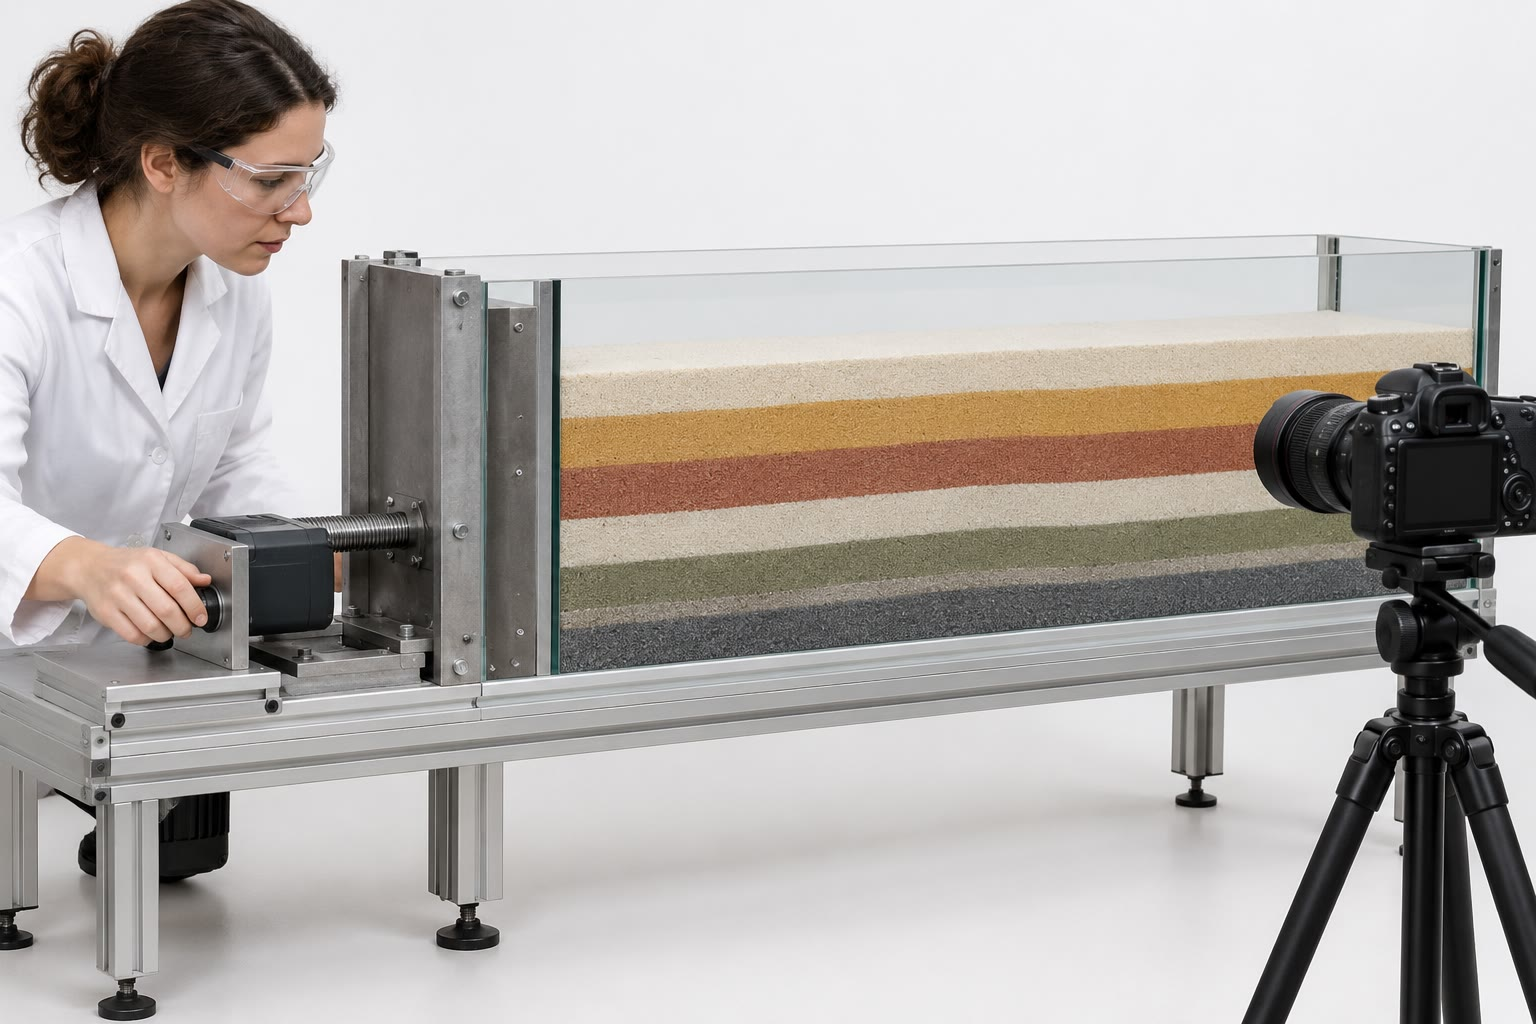
\includegraphics[width=\linewidth]{images/book5/ai/b3-sandbox-lab.jpg}

{\scriptsize Un modèle en bac à sable avant raccourcissement~: couches de sable colorées
dans une boîte à parois de verre, un mur motorisé à gauche, un appareil photo sur trépied
(Illustration générée par IA.)}
\end{minipage}
\end{inthelab}
% ledger: dsd83:taper

\section{Prismes réels}\label{sec:b3:orogenic-wedges:real}

Dans la zone active de plis et chevauchements de l'ouest de Taïwan, la pente de la surface, le
pendage du décollement et les pressions interstitielles sont tous connus, grâce à la topographie,
aux coupes sismiques et aux forages. Davis, Suppe et Dahlen s'en sont servis pour résoudre
l'\omterm{thm:b3:orogenic-wedges:critical-taper}{équation du biseau critique} pour déterminer la résistance du prisme, et ont trouvé $\mu = 1.03$
à l'intérieur et $\mu_b = 0.85$ à la base~: un frottement de Byerlee à la base, et un
prisme plus résistant que ses propres failles, car elles ne sont pas toutes orientées
pour glisser facilement. Avec ces deux coefficients, ils ont converti les biseaux observés
d'autres prismes actifs, sur terre et sous la mer, en rapports de pression interstitielle, et
ils les ont trouvés partout supérieurs à l'hydrostatique, en accord avec les forages. Ils ont aussi repéré
où la théorie cesse de s'appliquer~: le biseau chute brutalement là où les prismes
deviennent plus épais qu'environ \qty{15}{km}, profondeur à laquelle les roches riches en quartz
deviennent plastiques pour les géothermes courants, et la base n'obéit plus à une loi de frottement.
% ledger: dsd83:taper

Sur le front des Alpes occidentales, le Jura est un prisme de chevauchement à angle
étroit, de seulement 3 à \ang{4}. Son décollement se trouve surtout dans des couches
à halite d'âge triasique, et les fluides y ne sont pas surpressurisés~: la faiblesse
du sel explique à elle seule le biseau étroit. Au sud du Jura, là où les couches
triasiques ne contiennent pas de halite, le même front présente un biseau de 12 à
\ang{13}, avec un empilement d'écailles de chevauchement, bien que les pressions de fluide
mesurées y soient élevées. Dans les Alpes centrales, l'analyse du \omterm{def:b3:orogenic-wedges:critical-taper}{biseau critique} de la pente
de surface donne une résistance basale $\mu_b(1 - \lambda_b)$ (avec un petit terme de
cohésion) inférieure à 0.1, et même à 0.05 dans les évaporites et les schistes près du front,
cette valeur augmentant vers l'arrière-pays, avec des rapports de pression interstitielle
supérieurs à 0.54. La base d'un prisme est souvent bien plus faible que ne le prévoit la loi
de Byerlee, en raison de son type de roche et de ses fluides.
% ledger: deville21:jura, vonhagke14:alps

\section{Flux à travers un prisme}\label{sec:b3:orogenic-wedges:flux}

Un prisme à son \omterm{def:b3:orogenic-wedges:critical-taper}{biseau critique} croît par accrétion, à forme constante~: sa longueur
et sa hauteur augmentent ensemble. L'érosion retire de la roche à sa surface. Lorsque
les deux se compensent, le prisme conserve sa taille, et la roche le traverse.

\begin{proposition}[Bilan de flux en régime stationnaire]\label{prop:b3:orogenic-wedges:flux}
Un prisme de largeur $W$ suivant la direction de transport reçoit, par unité de longueur
de la chaîne, le flux d'accrétion $F_a = v h$, où $v$ est la vitesse de convergence et $h$
l'épaisseur de la couche entrante au-dessus du décollement. Il perd le flux érosif
$F_e = \bar e W$, où $\bar e$ est la vitesse d'érosion moyenne sur sa surface. Son aire
de section varie au taux $F_a -
F_e$~; en régime stationnaire, $\bar e = vh/W$.
\end{proposition}

\begin{proof}
Pendant une unité de temps, une longueur $v$ de la couche entrante, d'épaisseur $h$, passe
dans le prisme à travers son front, et l'épaisseur $e(x)$ est retirée en chaque
point de sa surface~; l'aire étant conservée, l'aire de la section varie de
$vh - \int_0^W e\,\mathrm dx = F_a - F_e$. En régime stationnaire, cette
variation est nulle.
\end{proof}

Avec $v = \qty{10}{mm/an}$, $h = \qty{4}{km}$ et $W = \qty{60}{km}$, la
vitesse d'érosion nécessaire au régime stationnaire est $\qty{0.67}{mm/an}$. L'exhumation, au
sens du volume de deuxième année, est l'enlèvement de la roche située au-dessus d'une
roche donnée~: en régime stationnaire, les roches atteignent la surface au rythme auquel l'érosion
l'abaisse, et le prisme les remonte depuis des profondeurs où elles étaient chaudes. Mesurer
la vitesse à laquelle cela se produit exige une horloge qui démarre à une température connue.

\section{Thermochronologie}\label{sec:b3:orogenic-wedges:thermochronology}

\begin{definition}[Thermochronologie, thermochronomètre]\label{def:b3:orogenic-wedges:thermochronology}
La \emph{thermochronologie}\index{thermochronologie} est l'utilisation
d'âges de refroidissement radiométriques pour dater le moment où une roche a
franchi une température donnée, et ainsi reconstruire son histoire thermique. Un
\emph{thermochronomètre}\index{thermochronomètre} est un couple formé d'un minéral et
d'une méthode de datation, assorti de sa température de fermeture~: par exemple
l'apatite avec la méthode (U--Th)/He, ou le zircon avec les traces de fission.
\end{definition}

Le tableau ci-dessous classe les principaux \omterm{def:b3:orogenic-wedges:thermochronology}{thermochronomètres} selon leur température de fermeture~;
les profondeurs supposent une température moyenne de surface de \qty{10}{\celsius} et un
gradient uniforme de \qty{30}{\celsius/km}. Une roche qui se refroidit au fur et à mesure
qu'elle est exhumée les franchit successivement, et ses âges croissent des
méthodes basse température vers les méthodes haute température. La physique des traces de fission et de
la diffusion de l'hélium, qui fixe ces températures, est présentée
au \cref{ch:b3:advanced-geochronology}.
\begin{center}
\small
% ledger: sueoka19:closure
\begin{tabular}{lcc}
\hline
\omterm{def:b3:orogenic-wedges:thermochronology}{thermochronomètre} & température de fermeture (\unit{\celsius}) & profondeur (\unit{km}) \\
\hline
(U--Th)/He sur apatite & 50--80 & 1.3--2.3 \\
traces de fission sur apatite & 90--120 & 2.7--3.7 \\
(U--Th)/He sur zircon & 160--200 & 5.0--6.3 \\
traces de fission sur zircon & environ 280 & 9 \\
\textsuperscript{40}Ar/\textsuperscript{39}Ar sur biotite & 350--400 & 11--13 \\
\textsuperscript{40}Ar/\textsuperscript{39}Ar sur muscovite & environ 425 & 14 \\
U--Pb sur zircon & supérieure à 900 & --- \\
\hline
\end{tabular}
\end{center}

Ces profondeurs ne sont qu'une première estimation, car l'érosion modifie le géotherme.

\begin{proposition}[Géotherme stationnaire avec érosion]\label{prop:b3:orogenic-wedges:geotherm}
Soit une roche remontant à vitesse constante $v$ à travers une couche d'épaisseur $L$ dont
surface ($z = 0$) est maintenue à $T_s$ et sa base à $T_L$, sans
production de chaleur. La température stationnaire vaut
\[
  T(z) = T_s + (T_L - T_s)\,\frac{1 - e^{-\mathrm{Pe}\,z/L}}{1 - e^{-\mathrm{Pe}}},
  \qquad \mathrm{Pe} = \frac{vL}{\kappa},
\]
et le gradient en surface vaut $\mathrm{Pe}/(1 - e^{-\mathrm{Pe}})$ fois
le gradient conductif $(T_L - T_s)/L$.
\end{proposition}

\begin{proof}
Une particule de roche à la profondeur $z$ remonte, vers les $z$ décroissants~: la
température qu'elle transporte évolue comme $\partial T/\partial t - v\,\partial
T/\partial z$, et l'équation de diffusion devient $\partial T/\partial t - v
T' = \kappa T''$. En régime stationnaire, $T'' = -(v/\kappa)T'$, donc $T' = C
e^{-vz/\kappa}$ et $T = T_s + C(\kappa/v)(1 - e^{-vz/\kappa})$, qui vérifie
$T(0) = T_s$. Imposer $T(L) = T_L$ fixe $C$ et donne la formule. En $z =
0$, $T' = (T_L - T_s)(\mathrm{Pe}/L)/(1 - e^{-\mathrm{Pe}})$.
\end{proof}

Pour $\mathrm{Pe} \ll 1$, le facteur tend vers 1~: la conduction l'emporte et
le géotherme reste droit. Pour $v = \qty{1}{mm/an}$ sur \qty{30}{km}, avec
$\kappa = \qty{e-6}{m^2/s}$, $\mathrm{Pe} = 0.95$ et le gradient en surface
passe de 30 à \qty{46}{\celsius/km}~: les isothermes se resserrent vers la
surface et chaque \omterm{def:b3:orogenic-wedges:thermochronology}{thermochronomètre} se ferme plus près de la surface.
% ledger: england:kelvin, earle:settings

\begin{definition}[Relation âge--altitude]\label{def:b3:orogenic-wedges:age-elevation}
La \emph{relation âge--altitude}\index{relation âge--altitude} d'un
\omterm{def:b3:orogenic-wedges:thermochronology}{thermochronomètre} est le tracé des âges de refroidissement d'échantillons prélevés sur une
plage d'altitudes, généralement le long d'une pente raide ou d'un profil vertical,
en fonction de leur altitude.
\end{definition}

\begin{proposition}[Pente de la relation âge--altitude]\label{prop:b3:orogenic-wedges:age-elevation}
Soit des roches remontant verticalement à vitesse constante $v$ sous une
topographie stationnaire, et soit l'isotherme de fermeture à l'altitude $e(x) = e_0 +
f\,h(x)$, où $h(x)$ est l'altitude de la surface et $0 \le f < 1$. Un échantillon
prélevé en surface à l'altitude $h$ a pour âge $t = (h - e)/v$,
et la \omterm{def:b3:orogenic-wedges:age-elevation}{relation âge--altitude} est une droite de pente
\[
  \frac{\mathrm dh}{\mathrm dt} = \frac{v}{1 - f}.
\]
Avec un isotherme plat, $f = 0$ et la pente vaut la vitesse d'exhumation.
\end{proposition}

\begin{proof}
La roche située aujourd'hui en surface en $x$ a franchi l'isotherme de fermeture juste
en dessous, à l'altitude $e(x)$, et s'est élevée de $h - e$ depuis, à la vitesse $v$~:
$t = (h - e_0 - fh)/v = ((1 - f)h - e_0)/v$. D'où $\mathrm dt/\mathrm dh =
(1 - f)/v$.
\end{proof}

\begin{omfigure}
\begin{tikzpicture}
\begin{groupplot}[group style={group size=2 by 1, horizontal sep=1.7cm},
  omrecord, width=0.47\linewidth, height=0.45\linewidth, title style={font=\small},
  legend style={font=\scriptsize, legend cell align=left}]
\nextgroupplot[title={(a) âge--altitude}, xlabel={âge (U--Th)/He de l'apatite (\unit{Ma})},
  ylabel={altitude au-dessus de la moyenne (\unit{km})}, xmode=log, xmin=0.1, xmax=10,
  log ticks with fixed point, xtick={0.1,0.2,0.5,1,2,5,10}, ymin=-1, ymax=1]
% computed in figdata/bachelor-3/age_elevation.py
\addplot[black, thick, densely dotted] table[x=a30, y=h] {figdata/out/bachelor-3-age_elevation-ages.dat};
\addplot[red!70!black, thick, densely dashed] table[x=a10, y=h] {figdata/out/bachelor-3-age_elevation-ages.dat};
\addplot[omDef, thick] table[x=a03, y=h] {figdata/out/bachelor-3-age_elevation-ages.dat};
\nextgroupplot[title={(b) l'isotherme de fermeture}, xlabel={distance (\unit{km})},
  ylabel={altitude au-dessus de la moyenne (\unit{km})}, xmin=0, xmax=40, ymin=-3.3, ymax=1.2,
  legend style={at={(0.5,0.03)}, anchor=south, legend columns=2}]
\addplot[black!70, very thick] table[x=x, y=h] {figdata/out/bachelor-3-age_elevation-iso.dat};
\addlegendentry{surface}
\addplot[black, thick, densely dotted] table[x=x, y=e30] {figdata/out/bachelor-3-age_elevation-iso.dat};
\addlegendentry{\qty{3}{mm/an}}
\addplot[red!70!black, thick, densely dashed] table[x=x, y=e10] {figdata/out/bachelor-3-age_elevation-iso.dat};
\addlegendentry{\qty{1}{mm/an}}
\addplot[omDef, thick] table[x=x, y=e03] {figdata/out/bachelor-3-age_elevation-iso.dat};
\addlegendentry{\qty{0.3}{mm/an}}
\end{groupplot}
\end{tikzpicture}

\par\smallskip{\small Exhumation stationnaire sous un relief sinusoïdal de
longueur d'onde \qty{20}{km} et amplitude \qty{1}{km}, pour trois vitesses,
styles de trait comme dans la légende de (b) (modèle du premier ordre~; couche de \qty{30}{km} d'épaisseur, surface à \qty{10}{\celsius},
\qty{30}{\celsius/km} sans érosion, $\kappa = \qty{e-6}{m^2/s}$, gradient
thermique atmosphérique \qty{6.5}{\celsius/km}, température de fermeture de \qty{65}{\celsius}). (a) Âge en fonction de
l'altitude~: les pentes valent 0.59, 2.5 et \qty{14}{mm/an}, et non 0.3, 1 et 3.
(b) L'isotherme à \qty{65}{\celsius} suit d'autant plus étroitement la topographie que
l'exhumation est rapide, car elle remonte plus près de la surface.}\label{fig:b3:orogenic-wedges:age-elevation}
\end{omfigure}
% ledger: earle:settings, england:kelvin, ussa76:layers, sueoka19:closure

Les isothermes ne sont pas plates sous un relief~: la surface est plus froide sur les sommets
que dans les vallées, d'un écart fixé par le gradient thermique atmosphérique, mais beaucoup moins que
dans la roche à la même altitude en profondeur, et les isothermes superficielles
suivent la topographie de façon atténuée. Pour une topographie sinusoïdale de
longueur d'onde $\Lambda$ et un gradient thermique atmosphérique $\Gamma$, une solution au premier ordre de l'équation
stationnaire donne
\[
  f = \frac{(G_0 - \Gamma)\,e^{-mz_c}}{G(z_c)},\qquad
  m = \frac{v}{2\kappa} + \sqrt{\Bigl(\frac{v}{2\kappa}\Bigr)^2 +
  \Bigl(\frac{2\pi}{\Lambda}\Bigr)^2},
\]
où $z_c$ est la profondeur de l'isotherme de fermeture sous la surface moyenne,
$G_0$ le gradient en surface et $G(z_c)$ le gradient en $z_c$ (admis~;
le script le vérifie). La perturbation s'amortit avec la profondeur sur
la distance $1/m$, au plus $\Lambda/2\pi$~: les \omterm{def:b3:orogenic-wedges:thermochronology}{thermochronomètres} basse température,
qui se ferment peu profondément, ressentent le plus le relief. La figure ci-dessus montre l'effet
pour l'apatite (U--Th)/He.
% ledger: sueoka19:closure, ussa76:layers

Un profil âge--altitude ne mesure la vitesse d'exhumation que là où
l'isotherme de fermeture est plane sous le relief. Ailleurs, elle la surestime d'un facteur $1/(1 - f)$, qui atteint
deux ou plus pour l'apatite (U--Th)/He dans un relief de longueur d'onde \qty{20}{km}.
Les âges issus de plusieurs \omterm{def:b3:orogenic-wedges:thermochronology}{thermochronomètres} sur les mêmes échantillons, et les modèles
thermiques du relief, permettent de le corriger.

\section{Exercices}

\begin{exercise}[$\star$]\label{exo:b3:orogenic-wedges:1}
Calculer $K$ et le rapport $\sigma'_1/\sigma'_3$ à la rupture pour un prisme
de $\phi = \ang{30}$.
\end{exercise}

\begin{exercise}[$\star$]\label{exo:b3:orogenic-wedges:2}
Un prisme de sable sec en modèle analogique ($\lambda = \lambda_b = 0$) possède $\mu = 0.6$
à l'intérieur et $\mu_b = 0.3$ à sa base. Calculer sa pente critique de surface sur une
base horizontale, puis sur une base à pendage de \ang{3}.
\end{exercise}

\begin{exercise}[$\star$]\label{exo:b3:orogenic-wedges:3}
Avec une surface à \qty{10}{\celsius} et un gradient de \qty{30}{\celsius/km},
vérifier les profondeurs du tableau des températures de fermeture pour l'apatite
(U--Th)/He, traces de fission de l'apatite et traces de fission du zircon. Quel
\omterm{def:b3:orogenic-wedges:thermochronology}{thermochronomètre} choisir pour dater l'exhumation depuis \qty{5}{km}~?
\end{exercise}

\begin{exercise}[$\star$]\label{exo:b3:orogenic-wedges:4}
Une \omterm{def:b3:orogenic-wedges:thrust-geometry}{rampe} haute de \qty{2}{km} a un pendage de \ang{30}. Calculer sa longueur horizontale et sa
longueur le long du pendage. De combien un banc du toit est soulevé une fois
qu'il a franchi toute la \omterm{def:b3:orogenic-wedges:thrust-geometry}{rampe}, et quel glissement amène la coupure du banc le plus bas
du pied de la \omterm{def:b3:orogenic-wedges:thrust-geometry}{rampe} jusqu'au \omterm{def:b3:orogenic-wedges:thrust-geometry}{palier} supérieur~?
\end{exercise}

\begin{exercise}[$\star\star$]\label{exo:b3:orogenic-wedges:5}
Avec les coefficients de Taïwan, calculer la pente critique de surface sur une base
à pendage de \ang{6} pour $\lambda = \lambda_b = 0.4$ et $0.9$. Que produit une
augmentation de la pression de fluide interstitiel sur un prisme qui se trouvait à son \omterm{def:b3:orogenic-wedges:critical-taper}{biseau critique}~?
\end{exercise}

\begin{exercise}[$\star\star$]\label{exo:b3:orogenic-wedges:6}
Un \omterm{def:b3:orogenic-wedges:thrust-folds}{pli de rampe} se forme au-dessus d'une \omterm{def:b3:orogenic-wedges:thrust-geometry}{rampe} haute de \qty{1.5}{km}~; un banc situé au-dessus du
\omterm{def:b3:orogenic-wedges:thrust-geometry}{palier} supérieur montre une aire excédentaire de \qty{6.0}{km^2}. Calculer le glissement. Un collègue
lit le même pli comme un \omterm{def:b3:orogenic-wedges:thrust-folds}{pli de décollement}, le banc se trouvant à \qty{3.0}{km} au-dessus
du décollement. Quel raccourcissement trouverait-il~?
\end{exercise}

\begin{exercise}[$\star\star$]\label{exo:b3:orogenic-wedges:7}
Prendre $\mu = 0.6$ à l'intérieur du prisme du Jura (biseau \ang{3.5}) et de celui situé au
sud (biseau \ang{12.5}), avec $\lambda = 0.4$ hydrostatique dans les deux, et
un pendage basal de \ang{2} pour les deux. Calculer la résistance basale $\mu_b(1 -
\lambda_b)$ que réclame chaque biseau, et la comparer au $0.85$ de Byerlee
à pression hydrostatique. Le résultat est-il compatible avec le décollement dans
l'halite sous le Jura~?
\end{exercise}

\begin{exercise}[$\star\star$]\label{exo:b3:orogenic-wedges:8}
La roche remonte à \qty{1}{mm/an} à travers une couche de \qty{30}{km} d'épaisseur, depuis
\qty{910}{\celsius} à sa base jusqu'à \qty{10}{\celsius} en surface, avec
$\kappa = \qty{e-6}{m^2/s}$. Calculer le \omterm{def:b3:lithosphere-thermal-models:peclet}{nombre de Péclet thermique}, le gradient en surface,
et la profondeur de l'isotherme \qty{65}{\celsius}. Comparer avec la profondeur
sans érosion.
\end{exercise}

\begin{exercise}[$\star\star$]\label{exo:b3:orogenic-wedges:9}
Deux échantillons prélevés sur la même pente, à 1200 et \qty{2000}{m}, ont des âges (U--Th)/He sur apatite de 3.4 et
\qty{4.6}{Ma}. Calculer la vitesse apparente d'exhumation. Un modèle
thermique du relief donne $f = 0.5$~: quelle est la vitesse réelle~?
\end{exercise}

\begin{exercise}[$\star\star\star$]\label{exo:b3:orogenic-wedges:10}
Montrer que, pour $\lambda = \lambda_b$, la pente critique de surface s'annule pour un
pendage basal $\beta^* = \mu_b/K$ qui ne dépend pas de $\lambda$. Calculer cette valeur pour
Taïwan. Que se passe-t-il pour un prisme dont la base présente un pendage plus fort~?
\end{exercise}

\begin{exercise}[$\star\star\star$]\label{exo:b3:orogenic-wedges:11}
Montrer que, pour une très grande longueur d'onde et une exhumation très lente, $f$ tend vers
$1 - \Gamma/G$, où $G$ est le gradient uniforme~; l'évaluer pour $G =
\qty{30}{\celsius/km}$ et $\Gamma = \qty{6.5}{\celsius/km}$. Quelle est alors la
pente de la \omterm{def:b3:orogenic-wedges:age-elevation}{relation âge--altitude}~? Pour $v = \qty{1}{mm/an}$ et les
valeurs de l'exercice~8 ($z_c = \qty{1.21}{km}$, $G_0 = \qty{46.5}{\celsius/km}$,
$G(z_c) = \qty{44.7}{\celsius/km}$), calculer $f$ pour des longueurs d'onde de 5 et
\qty{20}{km}.
\end{exercise}

\begin{exercise}[$\star\star\star$]\label{exo:b3:orogenic-wedges:12}
Un prisme croît à son \omterm{def:b3:orogenic-wedges:critical-taper}{biseau critique} $\alpha + \beta$ par
\omterm{def:b3:orogenic-wedges:accretion}{accrétion frontale} seule, sans érosion, à partir du flux $F_a$. Montrer que sa largeur croît selon
$W = \sqrt{2F_at/\tan(\alpha + \beta)}$. Avec $F_a = \qty{40}{km^2/Ma}$ et
un biseau de \ang{6}, quelle est sa largeur après \qty{2}{Ma}, et combien de temps
lui faut-il pour atteindre \qty{60}{km}~?
\end{exercise}

\section{Problème~: le front du prisme Kestrel}

\begin{problem}[{Problème du week-end --- le raccourcissement, la mécanique, le flux et
l'exhumation d'un prisme de chevauchement fictif}]
\label{pb:b3:orogenic-wedges:1}
% values: calc/ch10.py; critical_taper.py; age_elevation.py; fault_bend.py
La chaîne de Kestrel est le front fictif d'une chaîne de montagnes, une
ceinture de plis et chevauchements subaérienne, large de \qty{60}{km} et poussée à \qty{10}{mm/an} sur un
avant-pays dont la couche sédimentaire mesure \qty{4.0}{km} d'épaisseur au-dessus d'un
décollement dans les schistes. Son chevauchement frontal suit le décollement \qty{4.5}{km} sous la
surface, gravit une \omterm{def:b3:orogenic-wedges:thrust-geometry}{rampe} de pendage \ang{25} et court le long d'un \omterm{def:b3:orogenic-wedges:thrust-geometry}{palier} supérieur
situé à \qty{1.5}{km} de profondeur. Au front, la surface se trouve \qty{0.3}{km} au-dessus du
niveau de la mer et le décollement \qty{4.0}{km} en dessous~; \qty{60}{km} en arrière du
front, la surface culmine à \qty{2.4}{km} et le décollement se situe
\qty{8.2}{km} sous le niveau de la mer. Prendre, comme à Taïwan, $\mu = 1.03$ et $\mu_b =
0.85$, une masse volumique de roche de \qty{2500}{kg/m^3}, l'eau à \qty{1000}{kg/m^3} et
$g = \qty{9.81}{m/s^2}$.

\medskip\noindent\textbf{Partie I --- Géométrie du chevauchement.}
\begin{enumerate}
  \item Calculer la hauteur de la \omterm{def:b3:orogenic-wedges:thrust-geometry}{rampe}, sa longueur horizontale et sa longueur
        le long du pendage.
  \item De combien un banc du toit a-t-il été soulevé après avoir franchi
        l'ensemble de la \omterm{def:b3:orogenic-wedges:thrust-geometry}{rampe}~?
  \item Au-dessus de la \omterm{def:b3:orogenic-wedges:thrust-geometry}{rampe}, un banc reposant sur le \omterm{def:b3:orogenic-wedges:thrust-geometry}{palier} supérieur présente un excès
        d'aire de \qty{16.5}{km^2} au-dessus de son niveau régional. Calculer le rejet.
  \item Quel excès d'aire prévoir pour un banc plus superficiel~? Si le pli avait
        été interprété comme un \omterm{def:b3:orogenic-wedges:thrust-folds}{pli de décollement} reposant sur le décollement, le banc
        étant situé \qty{4.0}{km} au-dessus, quel raccourcissement aurait-on trouvé~?
  \item En arrière de la \omterm{def:b3:orogenic-wedges:thrust-geometry}{rampe}, une coupe sismique montre un \omterm{def:b3:orogenic-wedges:thrust-geometry}{duplex} de quatre écailles, chacune
        désormais longue de \qty{2.5}{km} le long du chevauchement de base, découpée dans des tranches
        longues de \qty{6.0}{km}. Calculer le raccourcissement absorbé par les écailles, et
        le comparer au rejet sur la \omterm{def:b3:orogenic-wedges:thrust-geometry}{rampe} frontale.
  \item Les écailles se sont formées en séquence. Laquelle est la plus jeune, et pourquoi le
        chevauchement de toit est-il plissé~?
\end{enumerate}

\medskip\noindent\textbf{Partie II --- Le biseau.}
\begin{enumerate}[resume]
  \item Calculer la pente de surface $\alpha$, le pendage de base $\beta$ et le
        biseau.
  \item Calculer l'épaisseur du prisme \qty{60}{km} en arrière du front. La théorie
        du prisme de Coulomb est-elle applicable~?
  \item Calculer $K$. Quelle pente de surface aurait un prisme sec sur cette base~?
  \item Quelle pente de surface aurait-il avec une pression de fluide hydrostatique dans
        le prisme et à sa base~? Le prisme est-il compatible avec celle-ci~?
  \item Résoudre l'\omterm{thm:b3:orogenic-wedges:critical-taper}{équation du biseau critique} pour $\lambda = \lambda_b$.
  \item Calculer la contrainte verticale, la pression de fluide et la pression
        hydrostatique à la base du prisme, \qty{60}{km} en arrière du front.
  \item Le drainage abaisse $\lambda$ à 0.7. Calculer la nouvelle pente critique de
        surface. Comment le prisme réagit-il~?
\end{enumerate}

\medskip\noindent\textbf{Partie III --- Le flux.}
\begin{enumerate}[resume]
  \item Calculer le flux d'accrétion par kilomètre de la chaîne.
  \item Quelle vitesse d'érosion moyenne maintient le prisme à l'état stationnaire~?
  \item Calculer le volume et la masse de roche érodée par an sur
        \qty{100}{km} de la chaîne.
  \item Si l'érosion cessait, à quelle vitesse le prisme s'élargirait-il au départ~?
  \item Si la moitié de la couche entrante était sous-placée sous l'arrière du
        prisme au lieu d'être accrétée à son front, la vitesse d'érosion moyenne
        à l'état stationnaire changerait-elle~? Où l'érosion se concentrerait-elle~?
\end{enumerate}

\medskip\noindent\textbf{Partie IV --- L'horloge.}
Prendre la couche épaisse de \qty{30}{km}, à \qty{10}{\celsius} à la surface moyenne
(\qty{2.0}{km} au-dessus du niveau de la mer) et \qty{910}{\celsius} à sa base, $\kappa
= \qty{e-6}{m^2/s}$, une température de fermeture de \qty{65}{\celsius} pour l'apatite
(U--Th)/He, un gradient de température avec l'altitude de \qty{6.5}{\celsius/km} et un relief de
longueur d'onde \qty{20}{km}. Cinq échantillons prélevés sur un versant donnent~:
\begin{center}
\small
\begin{tabular}{lccccc}
\hline
altitude (\unit{km}) & 1.30 & 1.65 & 2.00 & 2.35 & 2.70 \\
âge de l'apatite (U--Th)/He (\unit{Ma}) & 1.60 & 1.83 & 2.07 & 2.30 & 2.54 \\
\hline
\end{tabular}
\end{center}
\begin{enumerate}[resume]
  \item En prenant la vitesse d'érosion de la question~15 comme vitesse d'exhumation, calculer
        le \omterm{def:b3:lithosphere-thermal-models:peclet}{nombre de Péclet thermique} et le gradient de surface.
  \item Calculer la profondeur de l'isotherme de fermeture sous la surface moyenne et
        le gradient à cette profondeur.
  \item Avec un isotherme de fermeture plan, quel âge aurait un échantillon à l'altitude
        moyenne~? Comparer avec les données.
  \item Calculer $m$ et le facteur de déflexion $f$.
  \item Ajuster une droite aux données âge--altitude. Quelle vitesse d'exhumation apparente
        donne sa pente~?
  \item Corriger cette valeur de la déflexion de l'isotherme.
  \item Comparer avec la partie III et donner la vitesse d'exhumation du
        prisme Kestrel.
\end{enumerate}
\end{problem}
